Para implementar o armazenamento dos dados de uma mDL foi necessário desenvolver-se um \textit{parser} capaz de guardar os mesmos como objetos de dados BER-TLV (\textit{Basic Encoding
Rules} - \textit{Tag}, \textit{Length}, \textit{Value}), em hexadecimal, bem como recuperar esses dados para uma estrutura adequada. 

O principal objetivo deste \textit{parser} é automatizar o processo de conversão dos dados entre uma estrutura de dados e texto hexadecimal, e vice-versa. Para isso, basta indicar uma configuração básica ao \textit{parser}, escrita em \texttt{JSON}, sendo esta a estrutura seguida aquando da conversão.

A título ilustrativo, apresenta-se de seguida um exemplo básico deste tipo de configuração.

\begin{lstlisting}[language=json]
{
    "tag": "00",
    "length": "var",
    "content": {
        "var_name": {
            "tag": "01",
            "length": 4,
            "constraints": "[$N]{8}",
            "encode": "BCD"
        },

        "list_name": {
            "tag": "02",
            "length": "var",
            "content": {
                "number_of_entries": {
                    "tag": "03",
                    "length": "var",
                    "constraints": "(\\d{2}|1\\d{2})",
                    "decode": "int"
                },
                
                "list_var_name": {
                    "size_list": "number_of_entries",
                    "tag": "04",
                    "length": "var",
                    "constraints_func": "myFunction($DATA)"
                }
            }
        }
    }
}
\end{lstlisting}

\vspace{0.5cm}

Salienta-se a utilização das chaves \texttt{tag} e \texttt{length} que indicam, respetivamente, a \textit{tag} e o comprimento dos dados incluídos nessa configuração. O comprimento dos dados pode ser fixo (caso em que é indicado um inteiro correspondente à quantidade de \textit{bytes}) ou variável (\texttt{var}). No primeiro caso o comprimento é omitido da representação em hexadecimal, enquanto que no segundo caso esse valor tem de ser indicado. A \texttt{tag} é sempre apresentada na representação em hexadecimal e serve para identificar o elemento de dados que se está a ler quando se pretende converter essa representação para uma estrutura de dados.

Para além disso, a chave \texttt{content} indica a presença de variáveis das estruturas de dados (elementos de dados básicos) no respetivo valor. A variável é encontrada quando se alcança uma chave (diferente de \texttt{content}) cujo conteúdo não inclua nenhum \texttt{content}. É nesse ponto que os dados são, de facto, convertidos entre formatos. Relativamente ao exemplo de configuração ilustrativo apresentado, a respetiva estrutura de dados seria a apresentada na figura \ref{fig:impl_parser_01}, como \textit{input}.

Existem ainda outros elementos de validação que podem ser indicados relativamente aos elementos de dados básicos:

\begin{itemize}
    \item \texttt{constraints} -- Formato que o elemento de dados, como \textit{string}, deverá ter, recorrendo a expressões regulares. Este formato é validado, sendo apresentado um erro caso as restrições não se verifiquem. Salienta-se a possibilidade de utilização de alguns símbolos, que facilitam a representação de determinados tipos de caracteres:
    \begin{itemize}
        \item \texttt{[\$A]} : Caracter alfabético.
        \item \texttt{[\$N]} : Caracter numérico.
        \item \texttt{[\$S]} : Símbolo.
        \item \texttt{[\$D]} : Delimitador.
    \end{itemize}
    Estes caracteres podem ser combinados de várias formas. Por exemplo, pode-se representar um caracter alfanumérico ou espaço simples da seguinte forma: \texttt{[\$A\$N ]}.

    \item \texttt{constraints\_func} -- Invocação da função a utilizar para validar as restrições do elemento de dados associado. Note-se que esta função tem de ser implementada para cada caso específico. Possibilita-se a utilização da etiqueta \texttt{\$DATA} para aceder aos dados que se pretende validar.
    
    \item \texttt{encode} -- Formato utilizado para a codificação em hexadecimal, pelo que este componente poderá ser mais específico que os restantes. Pode tomar um dos seguintes valores (caso não se apresente nenhum destes, utiliza-se a codificação por defeito):
    \begin{itemize}
        \item \texttt{BCD}: \textit{Binary Coded Decimal} (utilizado sobre inteiros).
        \item \texttt{NO\_ENCODE}: Sem qualquer codificação (elemento de dados já se encontra no formato hexadecimal).
        \item \texttt{CATEGORIES\_ENCODE}: Codificação utilizada para as categorias de veículos.
        % TODO: Mudar nomes para DG_IDS_TAGS_ENCODE e DG_TAGS_ENCODE
        \item \texttt{DG\_TAGS\_ENCODE}: Codificação utilizada para uma lista de identificadores e \textit{tags} dos grupos de dados.
        \item \texttt{DG\_TAGS\_LIST\_ENCODE}: Codificação utilizada para uma lista de \textit{tags} dos grupos de dados.
        \item \texttt{BDB\_ENCODE}: Codificação de um \textit{Biometric Data Blocks}.
        \item \texttt{VERSION\_ENCODE}: Codificação da versão de um \textit{Biometric Data Block}.
        \item \texttt{DEFAULT}: Codificação por defeito (inteiro ou \textit{string} é convertido diretamente em \textit{string} hexadecimal).
    \end{itemize}
    
    \item \texttt{decode} -- Formato utilizado para a descodificar de hexadecimal para \textit{string} ou \textit{inteiro}. Note-se que a descodificação é efetuada de acordo com a codificação, mas os elementos básicos podem precisar de ser distinguidos entre os dois tipos referidos. Assim, pode tomar um dos seguintes valores (caso não se apresente nenhum destes, utiliza-se a descodificação para \textit{string}): \texttt{INT} e \texttt{STR}.
    
    \item \texttt{size\_list} -- Nome da chave (e da variável) que indica o número de elementos da respetiva lista. Note-se que a presença desta chave indica que o dado associado é uma lista, em que cada elemento tem o formato especificado nessa configuração.
\end{itemize}

Após esta análise do que é possível representar através da configuração \texttt{JSON}, é necessário perceber como esta é utilizada para converter estruturas de dados numa \textit{string} hexadecimal e vice-versa.

Relativamente à fase de codificação, salienta-se a função principal \texttt{encode}, que recebe como argumento a estrutura de dados a codificar e o nome do ficheiro \texttt{JSON} com a configuração. Esta função simplesmente lê o conteúdo da configuração e invoca a função recursiva \texttt{asn1\_encode}, passando como argumento a estrutura de dados e a respetiva configuração.

A função \texttt{asn1\_encode} é recursiva devido ao facto da configuração poder ter bastantes níveis de conteúdo, sendo necessário aplicar a mesma função para efetuar a codificação associada. Em termos gerais, esta função funciona conforme apresentado na figura \ref{fig:impl_parser_01}.

\begin{figure}[H]
    \centering
    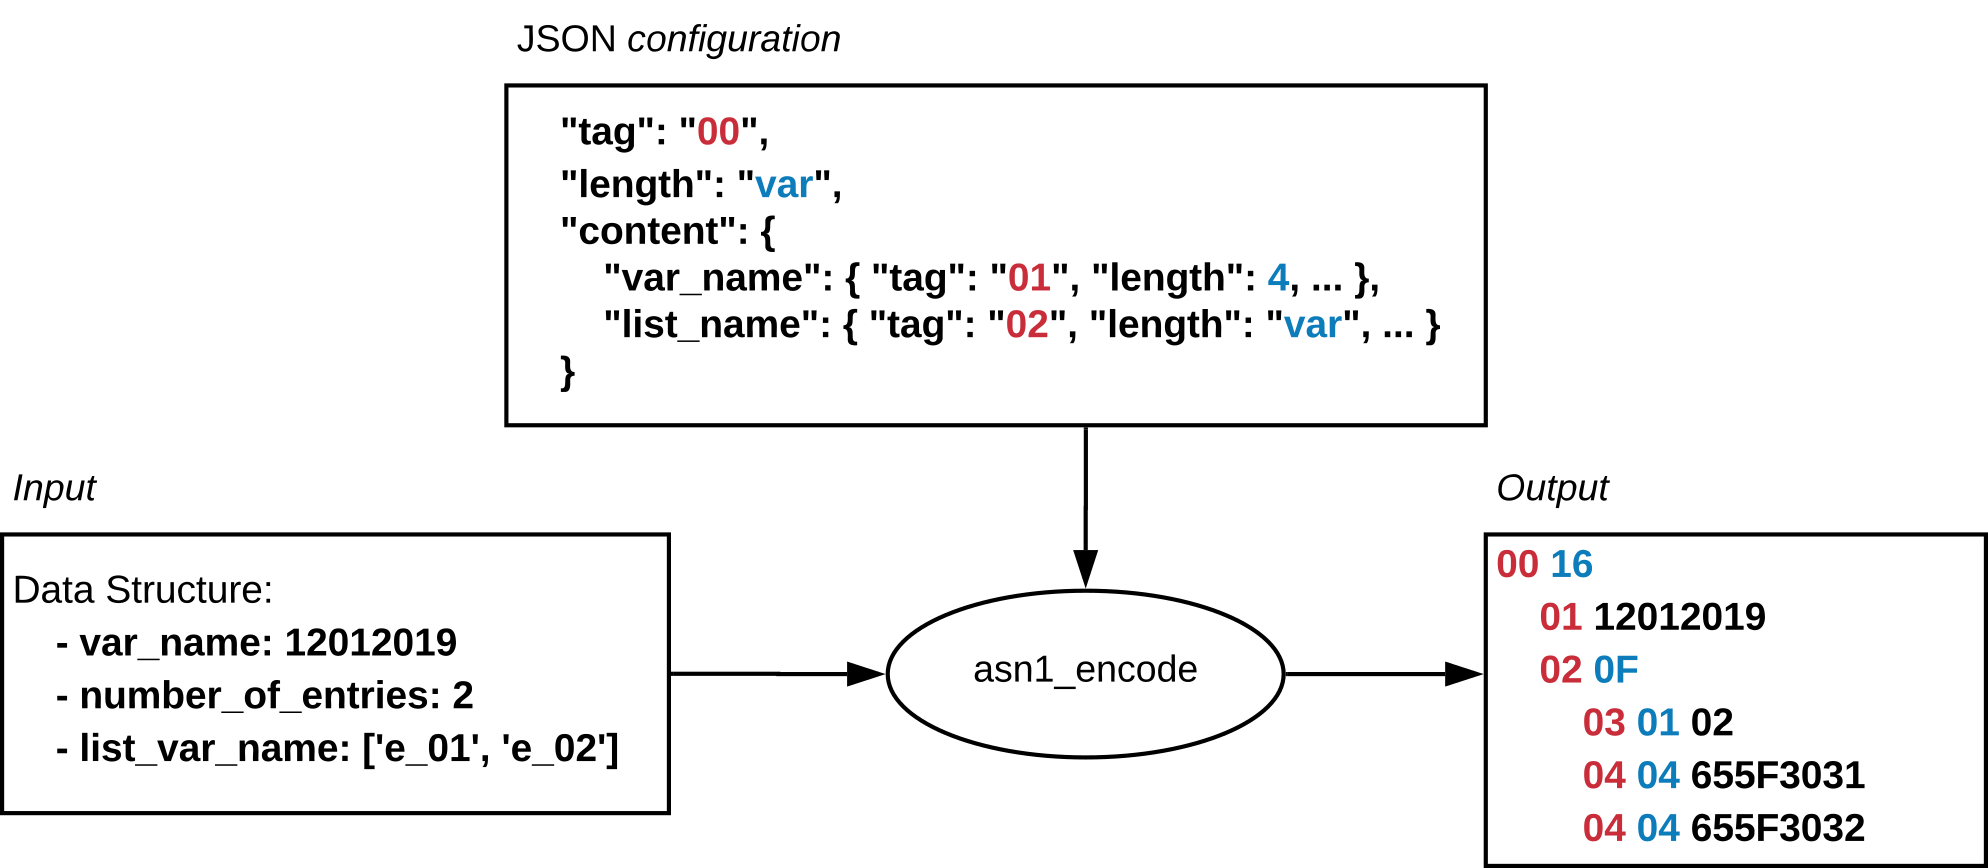
\includegraphics[width=0.95\textwidth]{impl_parser_01.png}
    \caption{Representação do funcionamento geral da função \texttt{asn1\_encode} (invocação principal).}
    \label{fig:impl_parser_01}
\end{figure}

Neste diagrama, bem como nos que se apresentarão de seguida, encontram-se realçadas a negrito as porções da configuração que são passadas como argumento à função indicada e as partes da estrutura de dados que são utilizadas. Para além disso, realçou-se as \textit{tags} a vermelho e os comprimentos a azul, de forma a permitir a sua fácil localização no \textit{output}. A formatação deste \textit{output} (espaçamento e cor) serve apenas para facilitar a perceção do mesmo, isto é, o \textit{output} real consiste apenas na \textit{string} simples em hexadecimal.

Como é necessário conhecer o comprimento dos dados associados ao \texttt{content} para indicar o mesmo na representação em hexadecimal, primeiro tem de se efetuar o \textit{parse} desse conteúdo. Assim, para cada chave dentro do \texttt{content}, a função \texttt{asn1\_encode} volta a invocar-se, com essa configuração, para obter os respetivos elementos de dados convertidos em hexadecimal. Assim, a função \texttt{asn1\_encode}, com os argumentos apresentados na figura \ref{fig:impl_parser_01}, efetua uma invocação recursiva com cada um dos seus \texttt{content}, conforme apresentado nas figuras \ref{fig:impl_parser_02} e \ref{fig:impl_parser_03}.

\begin{figure}[H]
    \centering
    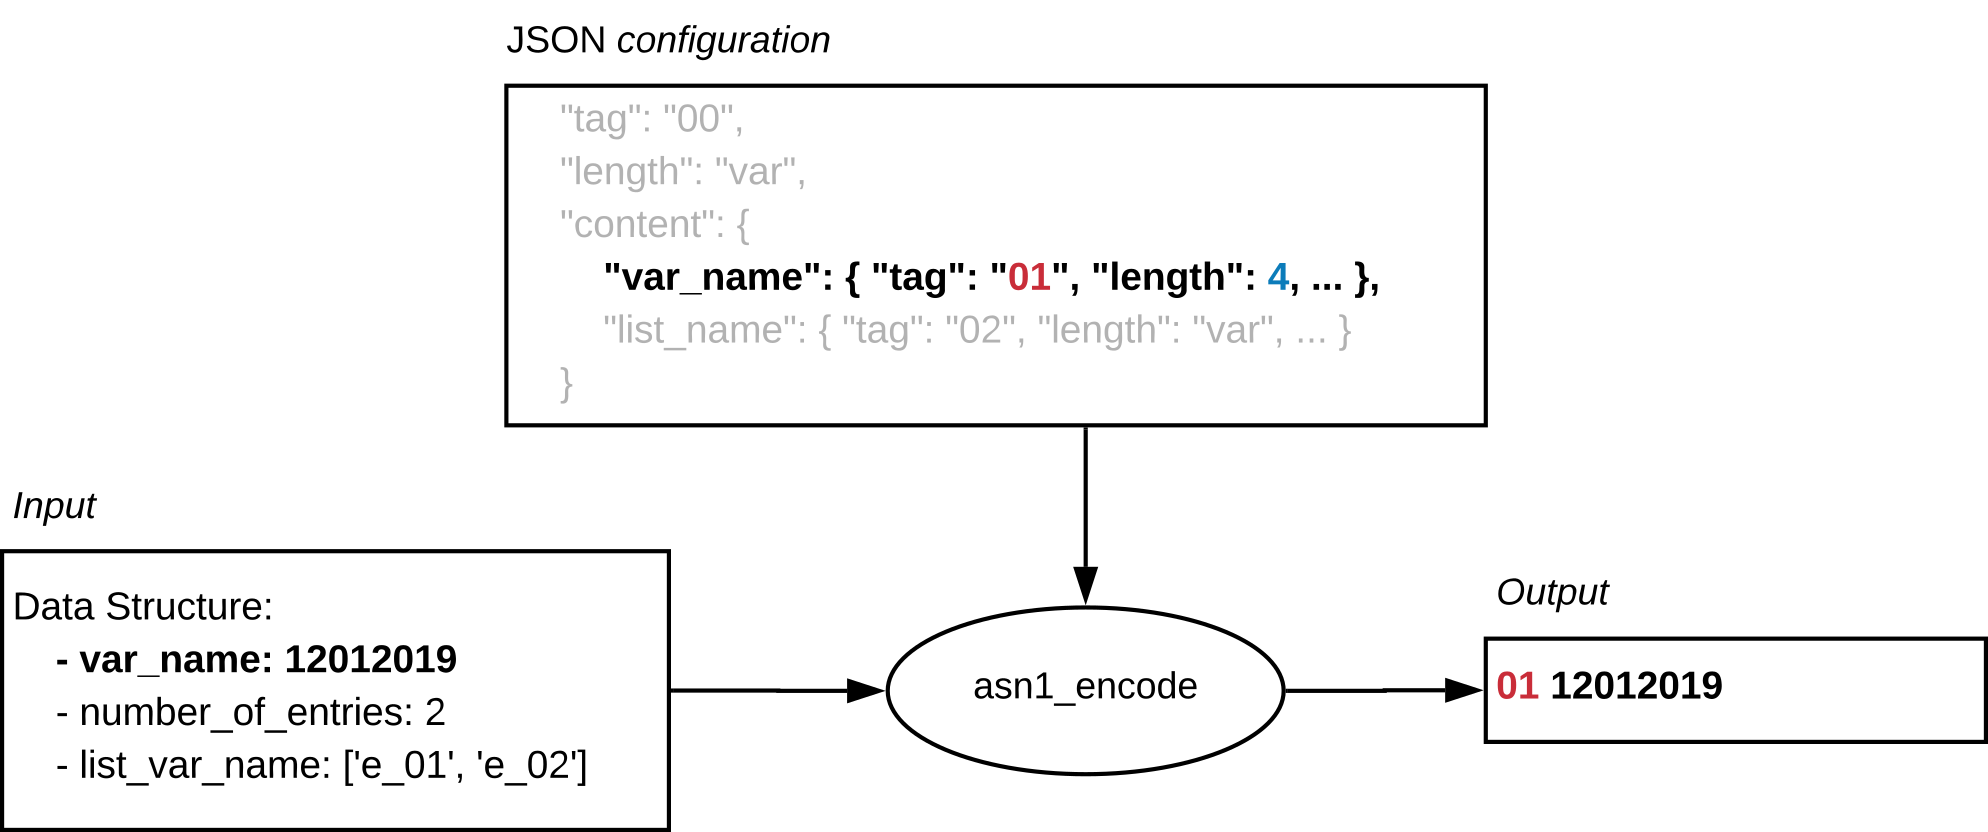
\includegraphics[width=0.89\textwidth]{impl_parser_02.png}
    \caption{Representação do funcionamento geral da função \texttt{asn1\_encode} (invocação para o conteúdo ``var\_name'').}
    \label{fig:impl_parser_02}
\end{figure}

\begin{figure}[H]
    \centering
    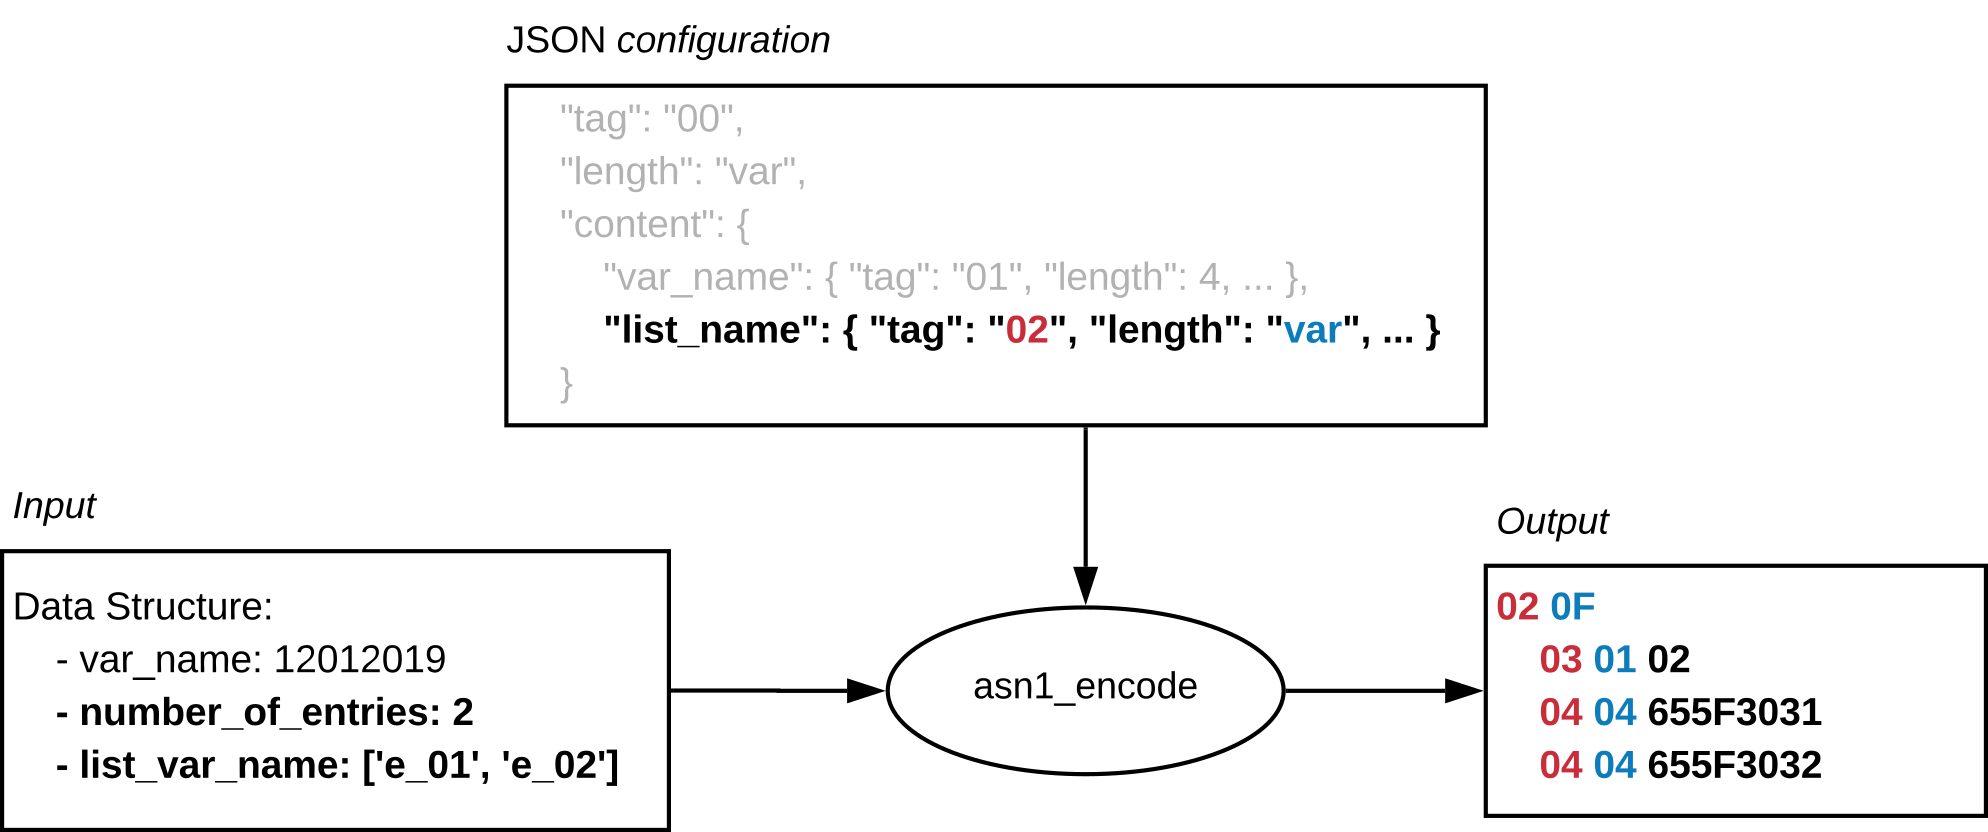
\includegraphics[width=0.89\textwidth]{impl_parser_03.png}
    \caption{Representação do funcionamento geral da função \texttt{asn1\_encode} (``list\_name'').}
    \label{fig:impl_parser_03}
\end{figure}


Relativamente à lista, processada na figura \ref{fig:impl_parser_03}, é notória a necessidade de novas invocações recursivas da função \texttt{asn1\_encode}. Para o conteúdo \texttt{number\_of\_entries}, o processamento é semelhante ao apresentado para a variável \texttt{var\_name}. Relativamente ao conteúdo \texttt{list\_var\_name}, a configuração realçada na figura \ref{fig:impl_parser_04} tem de ser utilizada para converter cada elemento da lista \texttt{list\_var\_name} do \textit{input}. Nessa figura apenas se representa a conversão para o primeiro elemento.

\begin{figure}[H]
    \centering
    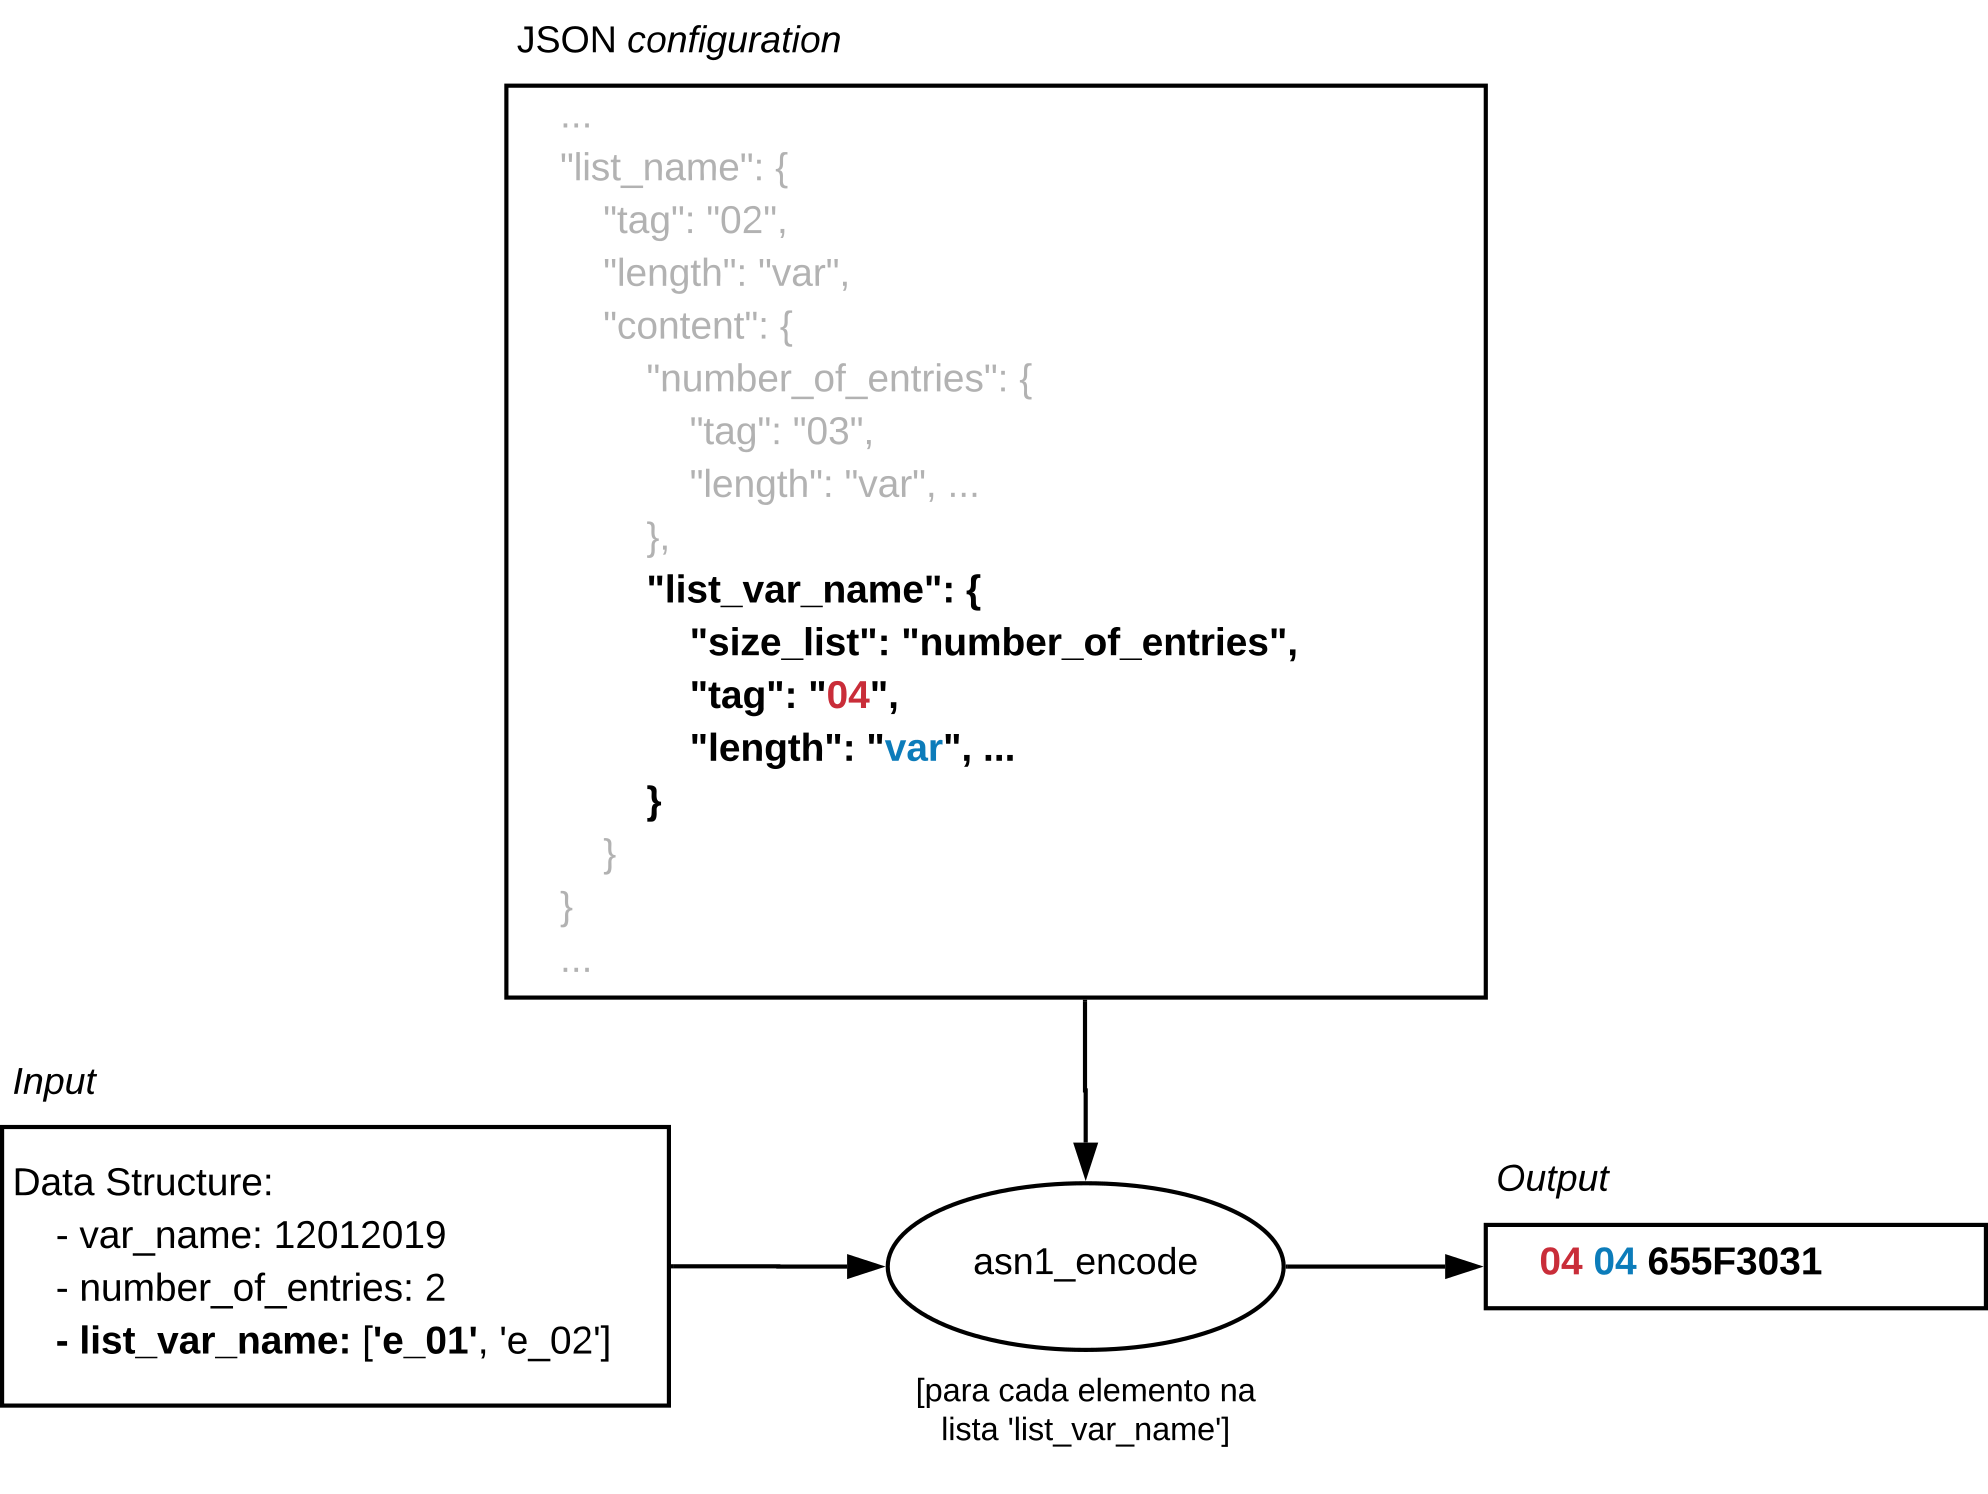
\includegraphics[width=0.89\textwidth]{impl_parser_04.png}
    \caption{Representação do funcionamento geral da função \texttt{asn1\_encode} (invocação para o conteúdo ``list\_var\_name'', dentro de ``list\_name'').}
    \label{fig:impl_parser_04}
\end{figure}

Para além destas listas simples, também é necessário, por vezes, armazenar listas compostas, em que cada elemento contém um determinado conjunto de dados. Para isso, pode-se utilizar uma configuração semelhante à que se apresenta de seguida.


\begin{lstlisting}[language=json]
{
    ...
    "compost_list_name": {
        "tag": "05",
        "length": "var",
        "content": {
            "number_of_entries": {
                "tag": "03",
                "length": "var",
                "decode": "int"
            },
            "list_var_name": {
                "size_list": "number_of_entries",
                "tag": "06",
                "length": "var", 
                "compost_content": {
                    "unused_name": {
                        "tag": "07",
                        "length": "var",
                        "content": {
                            "var_name_1": {
                                "tag": "08",
                                "length": 2,
                                "decode": "int"
                            }
                        }
                    },
                    "var_name_2": {
                        "tag": "09",
                        "length": "var"
                    }
                }
            }
        }
    }
    ...
}
\end{lstlisting}

\vspace{0.5cm}

Neste caso, utiliza-se a chave \texttt{compost\_content}, em vez de \texttt{content}, na configuração relativa ao elemento da lista. Desta forma, o \textit{parser} consegue distinguir se os dados associados correspondem a uma lista de elementos básicos (\textit{strings} ou inteiros) ou a uma lista de estruturas compostas.

Relativamente à descodificação da \textit{string} hexadecimal para uma estrutura de dados, esta é efetuada pela função principal \texttt{decode}, que recebe como argumentos a \textit{string} hexadecimal e o nome do ficheiro \texttt{JSON} com a configuração. Esta função invoca a \texttt{asn1\_decode} com a \textit{string} hexadecimal e a respetiva configuração, retornando o seu resultado (dicionário em que as chaves correspondem aos nomes das variáveis da estrutura original e os valores aos respetivos dados).

A função \texttt{asn1\_decode} também é recursiva, pelo motivo previamente apresentado em relação à função \texttt{asn1\_encode}. Neste caso, começa-se por extrair do início da \textit{string} hexadecimal a \textit{tag} e o respetivo comprimento (se este não for fixo, de acordo com a configuração). De seguida, extrai-se esse comprimento de \textit{bytes} do início da \textit{string} resultante, à qual se aplicará a função \textit{asn1\_decode}, se tiver conteúdo, ou se efetuará diretamente a conversão dos dados, caso contrário. Caso o comprimento da \textit{string} hexadecimal ultrapasse o comprimento esperado, é lançada uma exceção.

Assim, este é precisamente o processo inverso ao apresentado anteriormente, não se entrando, portanto, em tanto detalhe. Apenas se apresenta um diagrama representativo do funcionamento geral da função \textit{asn1\_decode}, na figura \ref{fig:impl_parser_05}.


\begin{figure}[H]
    \centering
    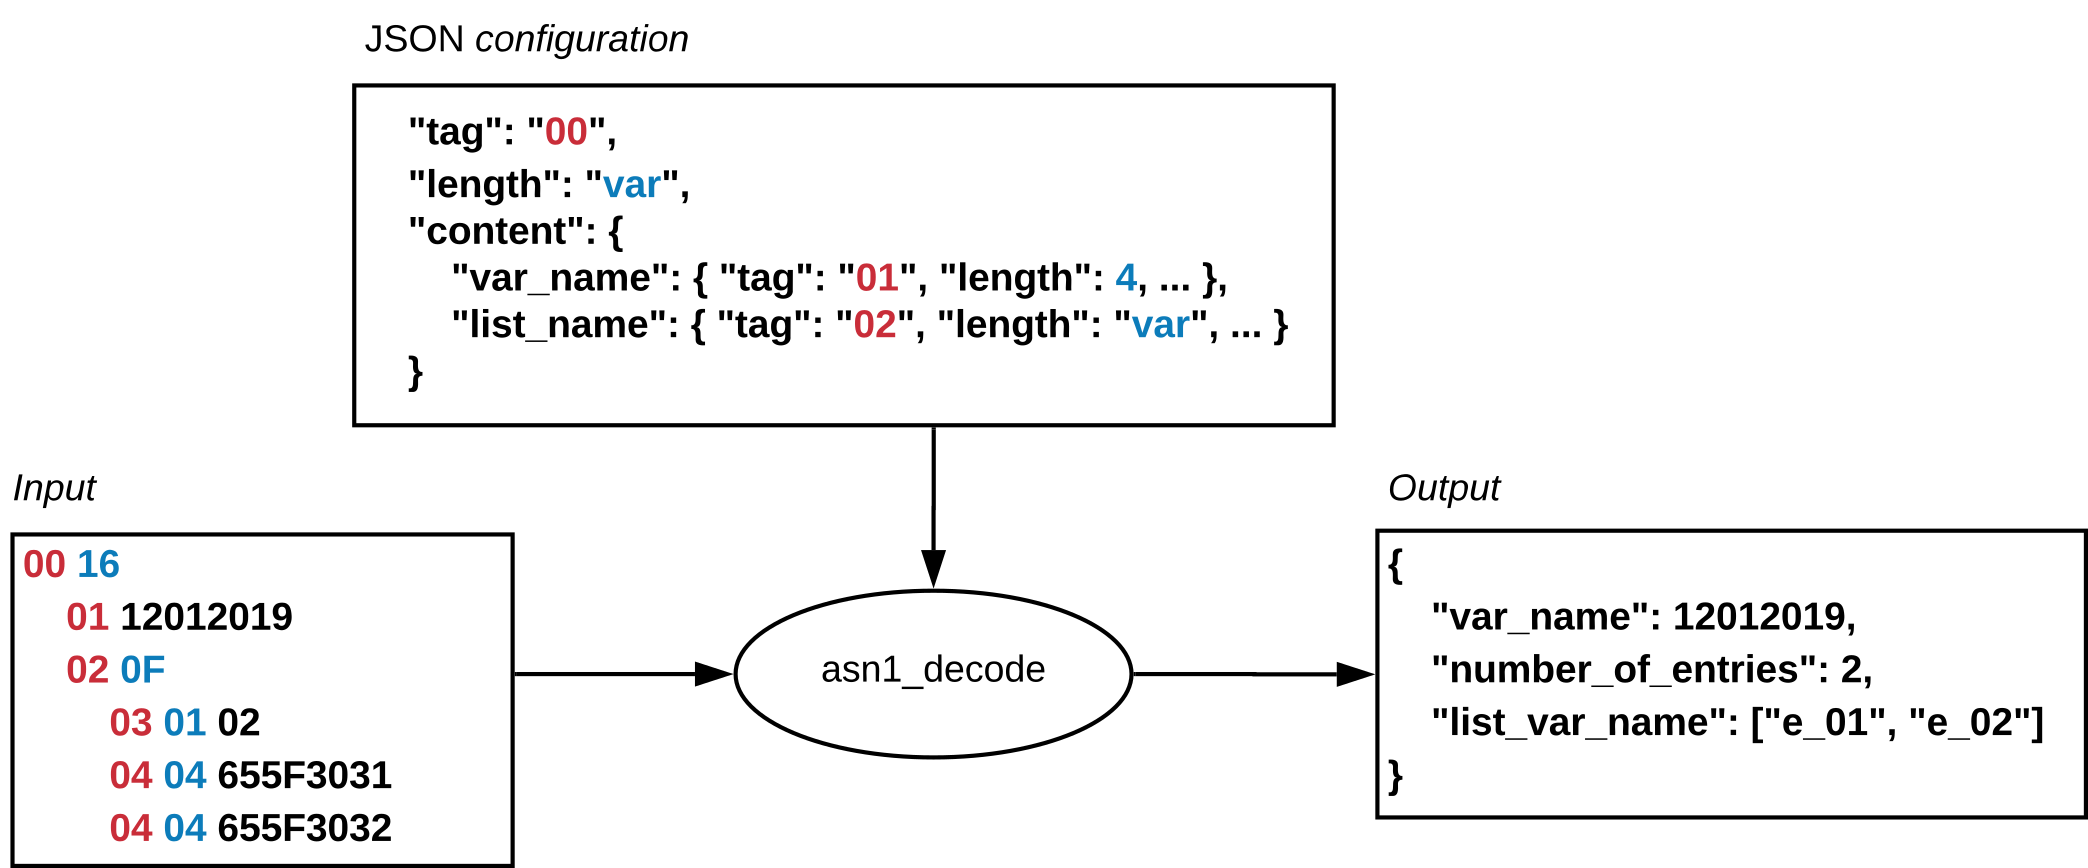
\includegraphics[width=0.95\textwidth]{impl_parser_05.png}
    \caption{Representação do funcionamento geral da função \texttt{asn1\_decode}.}
    \label{fig:impl_parser_05}
\end{figure}

Neste contexto, salienta-se apenas uma restrição relativamente ao comprimento dos dados armazenados para cada estrutura de dados, que não pode ultrapassar os 65 535 \textit{bytes}. A implementação foi efetuada desta forma, tendo em conta as regras de codificação do ASN.1 \textit{length}, especificadas no ISO/IEC 18013-2.

Por fim, tendo em conta toda a funcionalidade providenciada pelo \textit{parser}, este permitirá converter, de acordo com a especificação do ISO/IEC 18013, os dados dos \textit{data groups} em hexadecimal e vice-versa. Para além disso, também permite efetuar uma validação desses dados antes de os armazenar e após estes serem lidos.
